\chapter{Related Work}
\label{chapter:relatedwork}



The following sections detail the main related work researched in this thesis. In Section~\ref{ssec:num3} we explain the most used Automation Communication Protocols. Section \ref{ssec:num1} showcases both popular commercial home automation products, as well as academic automation solutions.
Section \ref{ssec:num2} follows with a description of some general purpose communication technologies, these technologies are widely available in mobile devices and as such play a important role.
 Finally, Section \ref{ssec:num4} presents commonly available sensors and how they can be applied to building automation and user comfort.
%Finally subsection \ref{ssec:num5} describes ...



\section{Building Automation Protocols} \label{ssec:num3}

Building automation systems are distributed control systems capable of monitoring and controlling a multitude of individual systems in a building. Usually they are used to control a building's heating, ventilation and air conditioning (HVAC), lighting, security and access control system (SAC).
The objectives of building automation are the reduction in energy consumption, operating cost, improvement of occupant comfort, and efficient operation of building systems.

\subsection{Zigbee}\label{zigbee_sub} \mbox{}\\

ZigBee \cite{livro_zigbee} is a short-range wireless communication protocol that uses a mesh-network in which the nodes are able to self organize. This provides an efficient way to integrate a large number of wireless devices in an automation scenario. ZigBee is a wireless personal area network (WPAN) and the devices may operate in several frequency bands (868 MHz, 915 MHz and 2.4 GHz). ZigBee main target is battery powered devices where low data rate, low cost and long battery life are the main requirements.

The ZigBee standard is developed by the ZigBee Alliance, a group of companies that maintains and publishes the ZigBee standard. 

The ZigBee standard has adopted IEEE 802.15.4 as its \ac{PHY} and \ac{MAC} protocols. Therefore, a ZigBee-compliant device is compliant with the IEEE 802.15.4 standard as well. 

ZigBee defines three device roles: the coordinator, the router and the ZigBee end device. The router is a device capable of relaying messages. If a device is the principal controller of a personal area network (PAN), it is called the coordinator. Finally, a ZigBee end device is a device that is neither a coordinator nor a router, it is the most simple device and has the ability to sleep to conserve power.


%There are two types of devices in an IEEE 802.15.4 wireless network: \textit{full-function devices} (FFD) \textit{and reduced-function devices} (RFDs). An FFD is capable performing any role in the network, but an RFD can only communicate with an FFD device. RFD devices are intended for simple applications such as turning on or off a switch.


Device networks must use one of two network topologies specified in IEEE 802.15.4: star and peer-to-peer. 

In a start topology, Figure \ref{zigbee1}, every device in the network can communicate only with the ZigBee coordinator. The advantage of star topology is that it is simple and packets go through at most two hops to reach their destination, the disadvantage is the coordinator can become a bottleneck.

In a peer-to-peer topology, Figure \ref{zigbee2}, each device can communicate directly with each other if the devices are close enough to establish a link. In a peer-to-peer network, only the coordinator or router devices can relay the messages. However a ZigBee end device can be part of the network and communicate with one device (a coordinator or router) in the network. This topology allows for greater range as packets can be routed across multiple routers.


\begin{figure}[h]
\centering
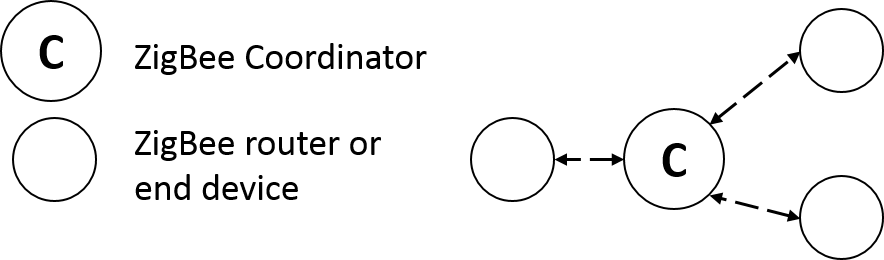
\includegraphics[width=0.7\textwidth]{Figures/zigbee1}
\caption{A Star Network Topology}
\label{zigbee1}
\end{figure}

\begin{figure}[h]
\centering
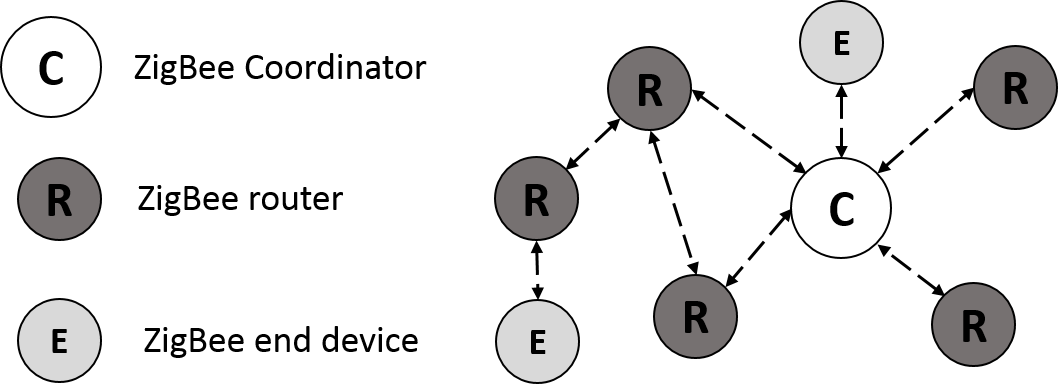
\includegraphics[width=0.7\textwidth]{Figures/zigbee2}
\caption{A Mesh Networking Topology}
\label{zigbee2}
\end{figure}

\begin{table}[h]
\centering
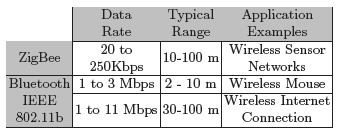
\includegraphics[width=0.6\textwidth]{Figures/comparison_}
\caption{Comparing ZigBee with bluetooth and 802.11b}
\label{table:comparison}
\end{table}

%\begin{table}[]
%\centering
%\begin{tabular}{c|c|c|c|}
%\cline{2-4}
%\multicolumn{1}{l|}{}                                                                                & \cellcolor[HTML]{C0C0C0}\begin{tabular}[c]{@{}c@{}}Data\\ Rate\end{tabular} & \cellcolor[HTML]{C0C0C0}\begin{tabular}[c]{@{}c@{}}Typical\\ Range\end{tabular} & \cellcolor[HTML]{C0C0C0}\begin{tabular}[c]{@{}c@{}}Application\\ Examples\end{tabular} \\ \hline
%\multicolumn{1}{|c|}{\cellcolor[HTML]{C0C0C0}ZigBee}                                                 & \begin{tabular}[c]{@{}c@{}}20 to\\ 250Kbps\end{tabular}                     & 10-100 m                                                                        & \begin{tabular}[c]{@{}c@{}}Wireless Sensor\\ Networks\end{tabular}                     \\ \hline
%\multicolumn{1}{|c|}{\cellcolor[HTML]{C0C0C0}Bluetooth}                                              & 1 to 3 Mbps                                                                 & 2 - 10 m                                                                        & Wireless Mouse                                                                         \\ \hline
%\multicolumn{1}{|c|}{\cellcolor[HTML]{C0C0C0}\begin{tabular}[c]{@{}c@{}}IEEE\\ 802.11b\end{tabular}} & 1 to 11 Mbps                                                                & 30-100 m                                                                        & \begin{tabular}[c]{@{}c@{}}Wireless Internet\\ Connection\end{tabular}                 \\ \hline
%\end{tabular}
%\caption{Comparing ZigBee with bluetooth and 802.11b}
%\label{table:comparison}
%\end{table}


 Table~\ref{table:comparison} compares Bluetooth, 802.11b (Wi-Fi) and ZigBee. ZigBee \cite{article:zigbee_survey} offers lower power consumption, less complexity and lower cost at the expense of less data rate.

Several attempts have been made to bring the power of zigbee to mobile terminals such as Android phones/tablets. In one example a Nokia phone running Symbian OS had a SD card with a zigbee radio attached, yet this approach only works for some models of phones since a side slot for a SD card is needed \cite{Sensing_Platform}.
In another project an Android phone communicated wirelessly with a computer (acting as a server) connected to a xbee module capable of communication with ZigBee devices or arduino boards with xbee modules \cite{article:zigbee_android}.

Commercially, Gateways\footnote{http://www.telegesis.com/products/zigbee-gateway-consumer-access-device/}$^{,}$\footnote{XBEE ZIGBEE GATEWAY}$^{,}$\footnote{Rainforest EAGLE Ethernet ZigBee Gateway} are used to communicate with ZigBee devices from a non ZigBee device, for instance an Android mobile device could interact with a ZigBee device by communicating with a ZigBee Wifi Gateway, the gateway would then relay the Android device messages to the ZigBee device.


\subsection{BACnet}\mbox{}\\


BACnet (Building Automation and Control Network) \cite{livro_automation,bacnet:artigo1,bacnet:bib,livro_automation2} is a standardized data communication protocol, evolved from the need for a standardized data communication protocol that would enable the various automation and control components in a building to communicate with each other, ensuring interoperability and manufacturer independence.

BACnet has a simple four layer architecture aimed to ensure the low cost development and production of BACnet devices. The Physical layer enables BAC devices to connect and transmit data. The data link focuses on point-to-point connections between two devices in a single network, organizes data into frames (or packets), regulates access to the medium, provides addressing, and handles some error recovery and flow control.
The network layer allows two or more subnets connected by a router using different data link layer options to communicate with each other, the focus of this layer is end-to-end connections across multiple networks. The BACnet standard is designed to connect devices only in one logical pathway, which simplifies the routing process in comparison to the Internet partial mesh topology, with multiple alternative paths.

%\begin{figure}[h]
%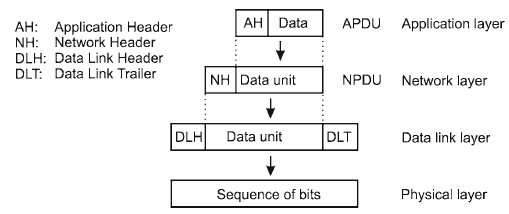
\includegraphics[width=0.7\textwidth, center]{bacnet_refazer}
%\caption{Bacnet data}
%\label{fig:bacnet_data}
%\end{figure}
%%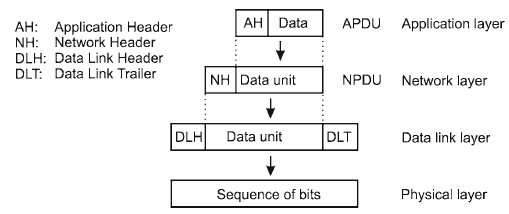
\includegraphics[width=0.5\textwidth]{bacnet_refazer}
%
%In BACnet the layers represented in Fig. \ref{fig:bacnet_data} encapsulate the data to create a message (data frame).
%The application header (AH) is added to the application data to form an application protocol data unit (APDU). This is forwarded to the network layer where a new network header (NH) containing global network address is added.
%The data link layer receives the previous data and adds a data link layer header (DLH) containing local network addresses. Finally the physical layer transfers the data over the transmission medium. These encapsulation steps are reversed at the receiver's side.  

BACnet data can be transmitted across several different types of networks, it provides four LAN technology options, one WPAN technology and one point-to-point protocol. The ones standardized were:  Master-Slave/Token-Passing (MS/TP); Point-to-Point (PTP); Ethernet; ARCNET; LonTalk and ZigBee.

The point-to-point (PTP) protocol is the only non LAN solution available in BACnet. It provides the means by which two remote devices can communicate directly with each other through a EIA-232 interface. The typical scenario could be to connect a dial-up modem to a remote building automation system. 

The first LAN alternative, Master-Slave/Token-Passing (MS/TP), is a simple protocol based on the use of EIA-485 (Electronic Industries Association) physical layer standard, suited for smaller control and operating units that do not require a fast transfer rate. An MS/TP network uses shielded twisted-pair cable as transmission medium.

The second alternative is Ethernet\footnote{https://en.wikipedia.org/wiki/Ethernet, last accessed on January 6$^{th}$, 2016} (ISO 8802-3), the highest performance LAN option. Nowadays office and industrial building are generally interconnected using Ethernet so it makes sense it would be used in building automation. Ethernet systems divide the stream data in small frames, each frame contains a source and destination address, as well as error-checking data.

The third option, ARCNET\footnote{https://en.wikipedia.org/wiki/ARCNET, last accessed on January 6$^{th}$, 2016}, is also LAN communication protocol. It became the American standard (ATA/ANSI 878.1). Unlike Ethernet, however, ARCNET is deterministic which means we know  the time it takes for the packet to arrive at its destination, which makes it good for use in industrial communications.

The fourth LAN protocol option in BACnet is LongTalk, it is a proprietary protocol developed by Echelon Corporation. LonTalk can be used in multiple different mediums by selecting appropriate compatible transceivers. The LonTalk protocol is low-cost, low-speed and has a limited message size of 128 octets.


The final protocol is ZigBee a WPAN protocol, described previously in section \ref{zigbee_sub}. After a joint effort by ZigBee and BACnet communities they aligned the two specifications\cite{bacnet_zig} so that compliant products can be designed that benefit from ZigBee's low-power, mesh wireless networking technology as well as BACnet's BAS data model and communications protocol.



BACnet uses 'objects' to provide a standard way of representing the functions of any device, each of which has a set of properties that characterize it. There are 25 standard object types. A device does not need to support all object types. 
BACnet defines 40 message types (services), that are divided into six categories: Object Access, File Access, Alarm and Event, Remote Device Management and Virtual Terminal.




\subsection{LonWorks}\mbox{}\\

LonWorks \cite{livro_automation2,livro_automation} is a networking solution for building automation and control networks. It is a proprietary solution developed by the American company Echelon. It can operate in both as a centralized building controller as well as in decentralized building control components.
LonWorks uses the LonTalk protocol which is a layered, packet-based, peer-to-peer communications protocol. LonTalk was designed to support many communication media and wiring topologies. Transmition media include twisted-pair, coaxial, and fiber-optic cable as well as radio systems that allow scalable transmissions speeds of up to 1.25 Mbit/s.

Figure \ref{fig:lon} describes the  LonTalk protocol architecture that uses the OSI Stack. The Physical Layer uses the above mentioned transmition media. The layers between the Data Link Layer and Presentation Layer are implemented using a Neuron chip.

Packets are routed using an routing algorithm. They can be addressed to a single device, to any group of devices, or to all devices. To support networks from two devices to tens of thousands of devices
the following types of addresses were defined:

\begin{itemize}
  \item Physical address: Every LonWorks device includes a unique never changing 48-bit identifier
called the Neuron ID.
  \item Device address: A LonWorks device is assigned a device address when it
is installed into a particular network. Device addresses are used instead
of physical addresses because they support more efficient routing of messages,
and they simplify replace failed devices.
  \item Group address: A group is a logical collection of devices within a domain.
Unlike a subnet, devices are grouped together without regard for their
physical location in the domain.
\item Broadcast address: A broadcast address identifies all devices with a subnet,
or all devices within a domain.
\end{itemize}

LonWorks offers three basic types of message delivery service and also supports authenticated messages. These message delivery services (listed below) allow trade-offs between reliability, efficiency and security:

\begin{itemize}
  \item Acknowledged messaging provides end-to-end guaranteed delivery. If acknowledgments are not received, the sender attempts the transaction again.
  \item Repeated messaging causes a message to be sent to a device or group of
any number of devices multiple times, without waiting for acknowledgments.
  \item Unacknowledged messaging send the message only once and does not expect a response.
  \item Authenticated service allows the receivers of a message to determine if the
sender is authorized to send that message. This is implemented by distributing 48-bit keys to the devices at installation time.
\end{itemize}


\begin{figure}[h]
\centering
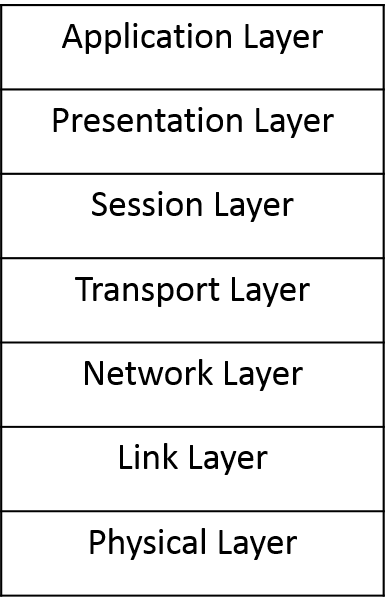
\includegraphics[width=0.3\textwidth]{Figures/lon_table}
\caption{LonTalk protocol architecture}
\label{fig:lon}
\end{figure}




%
%LonTalk \cite{livro_automation2}is a communication protocol developed by the company Echelon as part of the family of LonWorks protocols. LonTalj was designed to support many communication media and wiring topologies. Transmition media include twisted-pair, coaxial, and fiber-optic cable as well as radio systems that allow scalable transmissions speeds of up to 1.25 Mbit/s.


\subsection{Z-Wave}\label{zwave_sub}\mbox{}\\


Z-wave \cite{zwave}\cite{zigbeeAndZWave} is a proprietary wireless communication protocol, it allows interoperability between different manufacturers products. It is designed for control, monitoring and status reading application in residential and commercial environments.
Z-wave uses low powered RF communications technology operating in the sub-1GHz band that supports mesh networks without the need for a coordinator node.
Regarding data rates z-wave supports up to 100kbps, with AES128 encryption, IPV6 and multi-channel operation.

The Z-wav mesh enables any node to talk to other adjacent nodes directly or indirectly through available relays. If two nodes that want to communicate aren't within range, information can be exchanged with another node that both can access. The maximum number of hops supported is 4. Without any obstacles such as walls the range between two Z-Wave products is about 40 meters, this means the maximum range with 4 hops is roughly 200 meters.  


Primarily focused on monitoring and control functions in the home and  commercial facilities. Some solutions include lighting control, security, climate control, smoke detectors, door locks, security sensors, appliances, and remote controls.

\subsection{Summary}\mbox{}\\

The examined BAS were designed with low power consumption in mind. 

Platforms such as BAcNet and LonWorks require specialized professionals as well as personalized software and/or hardware to be configured. These solution present high installation costs. Newer solutions such as ZigBee and Z-Wave are present in many products and offer reduced installation and remodeling costs: various third-party vendors offer real time analysis and controls of these systems. One of the major problems with both ZigBee and Z-Wave is the lack of \ac{HVAC} products compatible with both standards, this means we probably won't use these standards to control an available \ac{HVAC} system.




\section{Home Automation Systems} \label{ssec:num1}

Home Automation is the Building Automation equivalent for the residential house.

The popularity of home automation has been increasing in recent years due to higher affordability and simplicity. Home automation  may include centralized control of lighting, HVAC (heating, ventilation and air conditioning), appliances, security locks of gates and doors and other systems.
Vendor solutions often rely in wireless technologies to connect the various devices, thus eliminating the need to rewire the house.

\subsection{Commercial Home/Office Automation Products}



\subsubsection{Philips hue}\mbox{}\\



The Philips hue\footnote{www2.meethue.com, last accessed on January 6$^{th}$, 2016} is a wireless lighting system developed by Philips\footnote{www.philips.com}. It is based on ZigBee LightLink\cite{zigbee:ZLL}, a low-power technology to control lights.

Figure \ref{fig:zll} illustrates the Philips Hue system, there are three main components: The lights, special light bulbs that meet the ZigBee standard; the bridge (gateway), that enables communication between a controller and the ZigBee lights; finally the controller, it can be the mobile app, the My Hue website or a smart light switch.


\begin{figure}[h]
\centering
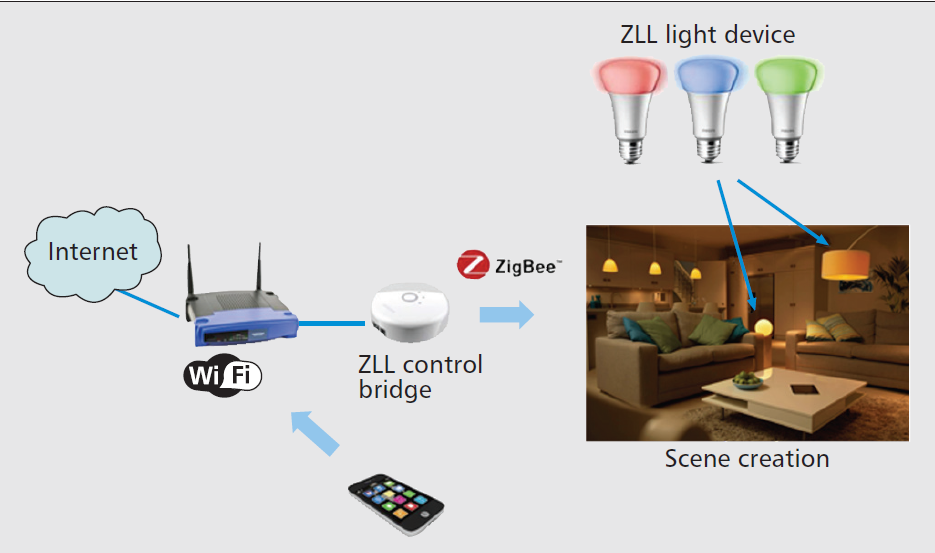
\includegraphics[width=0.7\textwidth]{Figures/philips_hue_refazer}
\caption{ZigBee Light Link devices communication through gateway}
\label{fig:zll}
\end{figure}

\subsubsection{WINK HUB}\mbox{}\\

Wink Hub is a home automation product developed by Wink\footnote{www.wink.com/}, it provides a unified automation platform capable of working with several different communication protocols: Wi-Fi, Bluetooth, Z-Wave, ZigBee, Lutron ClearConnect, and Kidde's RF-equipped devices.
As in other home automation solutions, the Wink Hub acts as a central controller being able to interact with the home devices, as well as users mobile apps.

\subsubsection{SmartThings}\mbox{}\\

Samsung offers a set of wireless SmartThings sensors and power outlet, they integrate with the SmartThings Hub to create a smart house.

SmartThings Hub is compatible with Z-Wave, Zigbee, and Wi-Fi radios. It can process video from compatible security cameras and can see live and recorded video from within the app. Moreover, you can have a connected camera begin recording when triggered by other SmartThings devices, such as a motion detector or a window sensor. 
The Hub allows the creation of IFTTT (If This Then That) recipes to make actions based on Web-based event triggers.

Sensors such as the Multi sensor can monitor whether doors, windows, cabinets or the garage door are open. Other devices like the Power Outlet can control lights, electronics and small appliances, they can even follow a schedule.


\subsubsection{Nest thermostat}\mbox{}\\


The Nest Learning Thermostat\footnote{https://nest.com/} is an electronic, programmable, and self-learning Wi-Fi thermostat. It uses machine learning algorithm to optimize  heating and cooling of homes. For the first weeks users have to regulate the thermostat in order to provide the reference data set. Nest can then learn people's schedule, at which temperature they are used to and when. 




\subsection{Academic Automation Systems}\mbox{}\\

Several academic home/office automation prototypes have been proposed over the years.

Kim Baraka and his co-authors proposed a home automation solution whose goal is not only to allow a user to control a house through a Android app but also to diminish the house energetic cost with the use a a scheduling algorithm \cite{academic:arduino1}. This prototype uses a Arduino Mega board acting as the central controller, the board is fitted with a Ethernet shield and a xbee module (wireless communication based on ZigBee protocol) that enable communication with the Android phone and other xbee devices in the home network. The Arduino board has the capability to schedule a list of task to ensure the total power used is not over a certain limit and that certain tasks are only scheduled when the energy price is cheaper, taking in account different day night power cost tariffs.
\mbox{}\\

This thesis was inspired by previous work done at IST Taguspark: PerOMAS (Personal Office Management and Automation System) \cite{peromas}. The proposed system consists of three main components: the Assistant, the Gateway and the Core.  The Assistant is present in every room and enables the occupant to take several actions that impact the room itself (lights, heating and cooling), the Gateways job is to collect data from the Assistants and take actions based on the collected data, e.g. controlling the lights of an hallway, turning them off if all the rooms in the hallway are empty, finally the Core is at the top of the hierarchy, its job can be to collect statistical data or perform action such as control a central boiler. 
Hardware wise these components were built using a Raspberry Pi Model B and several peripherals components such as LCD screen, temperature, humidity, luminosity sensors.

\mbox{}\\
Shiu Kumar proposed the use of a Arduino board with a Ethernet shield to provide connectivity to a Android app that enables the user to control a set of lights and electric devices (Air conditioner and fan)\cite{academic3}. The system is connected to several external sensors: temperature, smoke gas Sensor, passive infrared motion sensor that provides temperature monitoring, smoke detection and intrusion detection.
In the mobile app, besides manual buttons to turn on devices there is also voice activation support for switching functions. In the eventuality of fire or intrusion, email notification is sent to the user.
%Small comfort is added by the system, the ability to remotely turning on the air conditioning unit and the knowledge that in case of intrusion or fire we will be notified.


\subsection{Summary}\mbox{}\\

The above commercial solutions provide affordable but limited automation. Most home automation solution offer few supported standards. Most products specialize in lighting solutions but also add wireless video cameras, smoke detector and a few other devices. 

Some products are compatible with the IFTTT web-service, that allows devices to act on received messages from services such as gmail, twitter, weather and a few other. This functionality offers limited actions because most times the relevant triggers to an action are in the room (natural brightness, occupancy) and not in the cloud. For instance if there is sufficient natural sun light in a room the lights could be dimmed down or even turned off; If no one is using the room and certain appliances are turned on they should be turned off. 

In regards to the academic automation systems they focus more in energy saving  solutions, Kim Baraka and his co-authors\cite{academic:arduino1} focused in a proposed task scheduling algorithm that only provides monetary savings in the presence of different day night power cost tariffs. It did provide one energy saving proposal: turning lights off when luminosity exceeds a threshold.

PerOMAS\cite{peromas} provides important energy saving solutions such as: turning off the lights/HVAC if no occupant is detected, automatic HVAC on occupant presence and custom temperature values for different occupants. There is still room for improvement, one of the major problems faced is occupant detection. In the designed solution Bluetooth is used on occupants phones to detect room occupation. Most people don't keep their Bluetooth turned on, and a system should not depend on the possible existence of BT to detect the room occupation. 

The system proposed by \cite{academic3} focuses in controlling and monitoring the home. The notification system allows the user to be notified in the presence of an intrusion or fire detection.
No energy savings are achieved and no real increases in occupant comfort are present.



\section{General Purpose, Wireless Communication protocols} \label{ssec:num2}

Wireless communication allows the transmission of information over a distance without help of wires, cables or any other forms of electrical conductors. This freedom to connect devices without any physical connection has sparked the interest of the BA industry and standards development organizations, due to its flexibility in adding devices to the network and reduced installation costs. 
The technologies focused on below are the most used and available wireless technologies whose purpose is not just Building Automation, as seen in Z-Wave and ZigBee (\ref{zwave_sub} and \ref{zigbee_sub} respectively) both of which are wireless technologies. 


\subsection{Wireless Communications}

\subsubsection{Bluetooth (BT)}\mbox{}\\

Bluetooth is a wireless communication technology standard, IEEE 802.15.1, \cite{std_802.15.1,comunication:bt,comunication:bt_specification}, designed to exchange data over short distances between fixed and mobile devices and build WPAN. Originally develop by Ericsson \footnote{http://www.ericsson.com/} in 1994, it was created as an open standard to allow connectivity and collaboration between disparate products and industries.

BT runs in the 2.4 GHz Industrial, Scientific and Medical (ISM) band. Bluetooth employs frequency hopping techniques with the carrier modulated using one of three available modulations: Gaussian Frequency Shift Keying (GFSK), Differential Quadrature Phase Shift Keying (DQPSK) or differential phase-shift keying (8DPSK). The 8DPSK modulation scheme offers the highest bit rate possible of 3  Mbit/s. Many devices use the ISM band from microwave ovens to Wi-Fi. To avoid interference BT uses hopping carrier. A Bluetooth transmission only remains on one of its 79 channels for a short time, and if any interference is present the data will be re-sent later when the signal has changed to a different channel which is likely to be clear of other interfering signals.

Bluetooth operates based on a Master-Slave structure, where a master can communicate with up to seven slaves. All devices are synchronized with the master's clock and the slaves can only exchange data with the master.

The range of BT varies depending on the device power-class, higher power radios offer higher range. Figure \ref{fig:bt} describes the existing classes, Class 3 radios have a range of up to 1 meter, Class 2, found in mobile devices, 10 meters, and Class 1, primarily for industrial use cases, 100 meters.

\mbox{}\\
\textbf{Bluetooth Low Energy (BLE)}, is low-power variation of the original Bluetooth standard and was introduced as part of the Bluetooth 4.0 core specification. The main difference to traditional Bluetooth is Bluetooth 4.0's low power consumption. This enables applications to run on a small battery for four to five years. BLE devices still manage to transmit data at a reasonable rate of 1Mbit/s their focus in low power consumption, making then attractive to the Building Automation industry. 

BLE devices have a maximum range of 50 meters, the range can be increased by means of creating a mesh network of devices, to extend the range of BLE devices. 


\begin{table}[h]
\centering
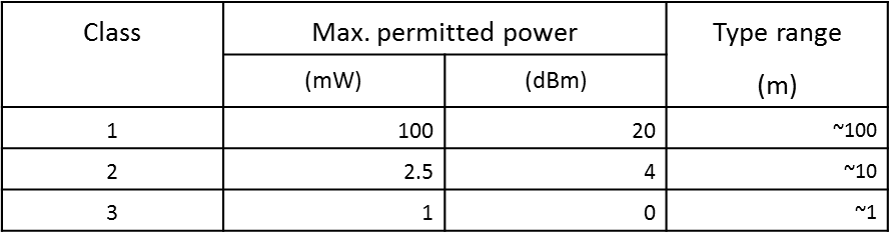
\includegraphics[width=0.7\textwidth]{Figures/bt_tabela1}
\caption{Available BT classes}
\label{fig:bt}
\end{table}


\subsubsection{Wireless fidelity (Wi-Fi)}\mbox{}\\

Wi-Fi is a WLAN based on the Institute of Electrical and Electronics Engineers' (IEEE) 802.11 standards \cite{IEEE_wifi,std_802.11,report_802.11}. It operates in the 2.4 and 5 Ghz frequency bands and uses CSMA/CA to control the medium access, offering data rates of up to 1.3 Gbp/s with the new IEEE 802.11ac revision.
To establish a network, one device called station (STA) connects to an other device called an Access Point (AP). An example for STA could be  a mobile device with Wi-Fi capability and the AP the router that usually delivers internet to the mobile device.
STAs associate and authenticate with the AP to get access to the network, forming a star topology. This topology is called an infrastructure Basic Service Set (BSS).

Wi-fi offer high-throughput at the cost of greater power consumption. Depending on the 802.11 protocol the maximum range in a indoor environment is between 35 (IEEE 802.11a, 802.11b, 802.11g, 802.11ac) to 70 meters (IEEE 802.11n).

\mbox{}\\
\textbf{Wi-Fi Direct} \cite{wifi_direct,wifi_direct2},  is a Wi-Fi standard that allows devices to connect with each other without requiring a wireless access point .
Unlike conventional Wi-Fi, which is primarily used for getting online, Wi-Fi Direct is intended for sharing media across platforms.

In Wi-Fi Direct the roles of AP and clients are dynamic, the device implementing AP-like functionality in the P2P Group is referred to as the P2P Group Owner (P2P GO), and devices acting as clients are known as P2P Clients. When two P2P devices discover each other they negotiate their roles (P2P Client and P2P GO) to establish a P2P Group. Once the P2P Group is established, other P2P Clients can join the group as in a traditional Wi-Fi network.

\mbox{}\\
\textbf{Security in Wi-Fi}, when using a wireless connection there is always a risk some third party is listening to the data exchanged between the mobile device and a server. A significant percentage of traffic consumed by mobile devices is not protected, a study\cite{internet_traffic} showed most traffic in mobile devices is web browsing (up to 58\%), in terms of Application layer protocols most traffic is HTTPS and HTTP.
The problem with using HTTP is you can't perform all operation like login or passing username and password or credit card information, because the sensitive data is sent in clear text and can be eavesdropped by anyone listening. The solution is to use HTTPS to ensure privacy and data integrity, HTTPS consists of communication over Hypertext Transfer Protocol (HTTP) within a connection encrypted by Transport Layer Security (TLS).



\subsubsection{IEEE 802.15.4}\mbox{}\\

IEEE 802.15.4 standard\cite{livro_zigbee} specifies the physical layer and media access control for  low-cost and low-rate wireless personal area networks (LR-WPANs).
There are three frequency bands in the latest version of IEEE 802.15.4: the 868 MHz band is used in Europe, the 915 MHz band is mainly in North America, whereas the 2.4 GHz band is used worldwide.

Figure \ref{fig:802.15.4}, details the ways these three frequency bands are used in the IEEE 802.15.4 standard.
The mandatory 868/915 MHz bands offer very low data rates (20 Kbps and 40 Kbps, respectively). In 2006 two optional PHY modes were introduced they achieve the 250 Kbps data rate at the 868/915 MHz bands.
Devices typical range is 10m, although a larger range is possible thanks to peer-to-peer networks between devices.

There are two types of devices in an IEEE 802.15.4 wireless network: full-function devices(FFDs) and reduced-function devices (RFDs). An FFD device can take three different roles: coordinator, PAN coordinator, and device. A coordinator is an FFD device that is capable of relaying messages. A PAN coordinator is the principal controller of a personal area network
(PAN). If a device is not acting as a coordinator, it is called a device .

An FFD is capable of performing any role in the network. An RFD has limited capabilities. FFD devices can communicate with any other device in a network, but an RFD can talk only with an FFD device. 


IEEE 802.15.4 defines four MAC frame structures: data, acknowledgment, beacon and MAC command frames.

The beacon frame is used to synchronize the clock of all the devices within the same network. The data and acknowledgment frames are used to transmit data and accordingly acknowledge the successful reception of a frame. The MAC commands such as requesting association or disassociation with a network are transmitted using a MAC command frame.



\begin{figure}[h]
\centering
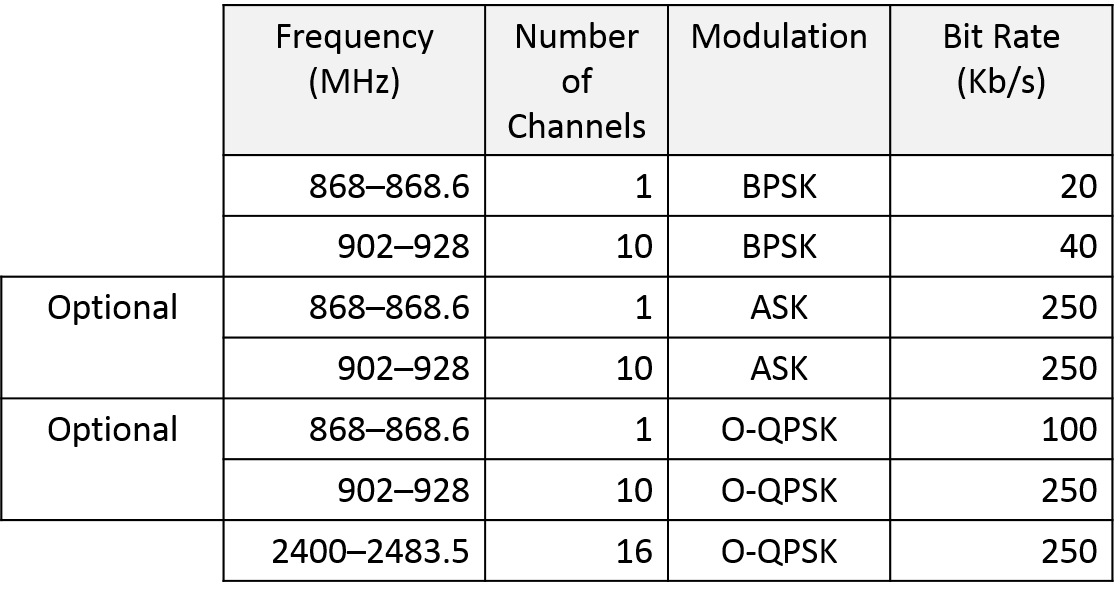
\includegraphics[width=0.7\textwidth]{Figures/802_15_4}
\caption{IEEE 802.15.4 Data Rates and Frequencies of Operation}
\label{fig:802.15.4}
\end{figure}


\subsection{Summary}\mbox{}\\

The examined wireless technologies offer alternatives to the ZigBee and Z-Wave presented previously, technologies like Bluetooth and especially Wi-Fi are used today for a variety of different ends, making both technologies accessible to most consumers.

Technologies such as Wi-Fi offer greater data transfer rates at the expense of greater power consumption: Wi-Fi can be used in BA if energy consumption costs aren't the major concern. Bluetooth Low Energy is a efficient wireless communication technology. Some lighting products are starting to take advantage of this technology commonly found in smartphones.

IEEE 802.15.4 based protocols offer low power wireless communications very attractive to BAS, however the lack compatible smartphone devices able to directly communicate using 802.15.4 create the necessity of using gateways to be able to communicate with such devices.  




\section{Sensors and their application in Automation Systems} \label{ssec:num4}\mbox{}

Sensors such as temperature or motion detection sensors provide information to Automation Systems, allowing them to respond to changes in the environment in which they are deployed. For instance a temperature sensor inside a room is able to relay the room temperature to the Automation System, which depending on the temperature values may turn on or off an air or heating unit to make the room more comfortable to the user.
Other sensors such as an ambient light sensor, can be used to save energy, for instance in a very bright day if no one is present in the room the blinds can be closed to prevent extra light from heating the room, this keeps the room colder and when the occupant arrives the room would be more comfortable, perhaps there would be no need to use a cooling unit saving in power costs.
%In the following paragraphs there is a description of some widely available sensors and some common application of those sensors in building automation.



\subsection{Sensors available in Android tablet/phone devices}\mbox{}\\

Sensor data is important for an Automation System as seen in the above examples. Regarding to this thesis main objective, the use of an Android device such as a tablet to act an a Building Automation Component, the following paragraphs provide a description of the sensors available in an Android mobile device \cite{android:sensors} and how we can leverage these sensors in order to build our automation system.

\textbf{Light Sensor}, measures the ambient light level;

\textbf{Pressure Sensor}, measures the ambient air pressure in hPa or mbar;

\textbf{Proximity Sensor}, measures the proximity of an object in cm relative to the view screen of a device;

\textbf{Ambient Temperature Sensor}, measures the ambient room temperature in degrees Celsius (\symbol{176} C);

\textbf{Magnetic Field Sensor}, measures the ambient geomagnetic field;

\textbf{Relative Humidity Sensor}, measures the relative ambient humidity in percent.

Besides the above sensors there are a few other described in \cite{android:sensors} but they provide data relative to the device itself such as rotation or accelerometer and at the moment we don't see how to take advantage of those sensors since the device will be stationary.

Furthermore an Android tablet/phone provides a camera, microphone and speakers. These will also be leveraged in our automation system.



\subsection{Sensor application in Automation Systems}\mbox{}\\

\subsubsection{Occupancy Detection}\label{ocupacy_detection}\mbox{}\\

Human behavior influences the amount of energy a building requires. Depending on the occupant behavior, the building's energy cost can increase or decrease by one-third of its design performance \cite{ocupancy2}. 
By knowing and tracking when a room is occupied, we can provide the system with relevant information that in turn my help in taking important actions such as switching off the lights if no one is present. 

There are several different methods to determine if a person is in the room, they range from Radio Frequency Identification (RFID), Passive Infrared (PIR), Vision-based, Wi-Fi and Bluetooth, among other \cite{ocupancy3}.

Yuvraj Agarwal and his co-authors proposed using a mixture of PIR sensor and a simple magnetic contact switch to track when the door opens and closes, this solution provides better result in regard to a PIR only solution\cite{ocupancy1}.

Using Wi-Fi it is possible to estimate the number of occupants in the area. Occupants usually have mobile devices connected to the building's Wi-Fi, by knowing the devices currently connected to the AP it is possible to estimate their relative location. Furthermore since it does not require additional equipment, it is an economic solution.
Sentinel uses a Remote Authentication Dial In User Service (RADIUS) server to provide centralized Authentication, Authorization, and Accounting \cite{wifi_ocupancy}. By using the logs provided by RADIUS the solution Sentinel is able to keep records on the occupancy of an area. 
Besides the Wi-Fi solution presented before one other alternative could be to use the Received Signal Strength (RSS) to determine the physical location of the mobile device\cite{wifi_ocupancy2}. This approach would require someone to go around the building mapping the signal strength in various points.

A camera and image analysis software are able to identify movement between video frames. Noise detection could also provide valuable input to determine occupation, yet it is less reliable as external sounds could induce false positive occupant detection.

\subsubsection{Auto Dimming light}\mbox{}\\

Some of the light bulbs available in the market can have built-in or external dimming. These lights have the ability to lower their light intensity and save energy.
By using an Light Sensor to measure the light level of a room and dimming lights it is possible to achieve saving in light energy, a study \cite{sensor_app_lights} showed saving of 10-20\% compared to full lighting by using dimming lights with a restriction that ensured the dimming could not go below 50\%. Saving could go up 16-32\% had the dimming to zero been allowed.


\subsubsection{Adaptive Heating/Cooling}\label{related:adaptive_heating}\mbox{}\\


Several studies show room temperature could influence productivity, Olli Seppanen and his co-authors developed an initial quantitative relationship between work performance and temperatures within and above the comfort zone\cite{temperature_survey}. Data collected from nine previous studies show the range of temperature in which people are most productive is between 22\symbol{176}C and 25\symbol{176} C. For temperatures between 25\symbol{176} C and 33\symbol{176} C they developed a model to measure the relationship between decrement in productivity P in \% and
temperature T in \symbol{176} C: 

P (\%) = [2 x (T,\symbol{176} C)] - 50 


\mbox{}\\
According with the American Society of Heating, Refrigerating, and Air Conditioning Engineers (ASHRAE), building occupant temperature comfort can be achieved for at least 80\% of occupants\cite{std_ASHRAE_55} by following the temperature range and humidity described in table \ref{tab_temperature}.

 
By using a temperature sensor within the room, the HVAC can be custom suited to the room itself. As different rooms within the same building have different temperature operation needs. If a building HVAC is turned on across the entire building uniformly, having the same temperature no matter the actual needs of the rooms and their occupants, there could be eventual comfort problems and excessive power consumption. A room with bright sun light can have a higher temperature than the room next to it without a window. Taking advantage of the fact that not all rooms have the same temperature requirements it is possible to save energy by only using the HVAC to keep the temperature within the room to human comfort levels or by not using ventilation if no occupant is present in the room and he is not expected to return soon.




\begin{figure}[h]
\centering
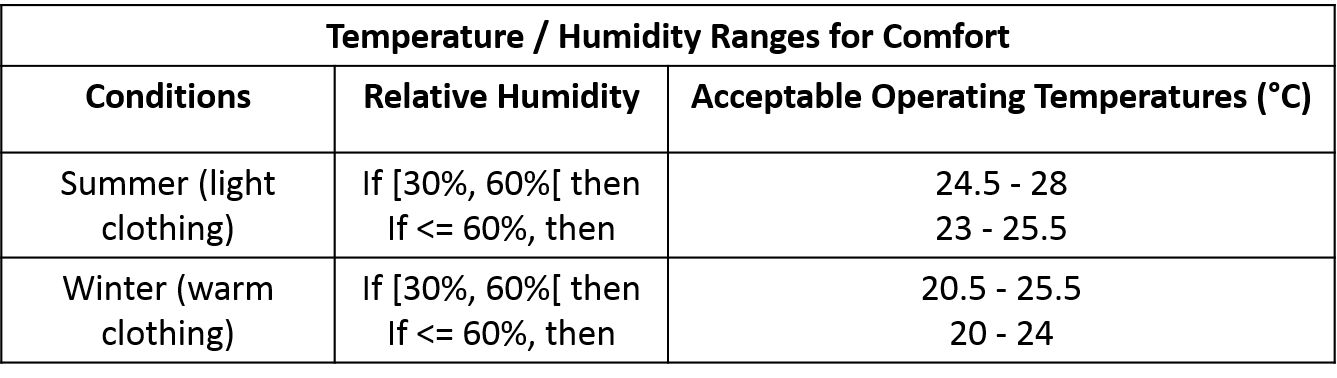
\includegraphics[width=0.7\textwidth]{Figures/tabela_temperatura}
\caption{Temperature / Humidity Ranges for Comfort}
\label{tab_temperature}
\end{figure}


\subsubsection{Monitoring/Security Systems}\mbox{}\\

The sense of security is important. By knowing our home or private work space is being monitored while we are not present we have one less stress factor to worry about.
In office buildings there are systems with a camera always recording (CCTV)\cite{livro_automation2} and a human monitoring the video stream. There are also other solutions that integrate sensor as well as image processing algorithms\cite{video_survailance1} to detect motion in video frames and warn the owner without the need of human monitoring. 




\subsection{Summary}\mbox{}\\

Sensors can have important contributes to Building Automation Systems. The above sensor applications can provide higher comfort to the occupants of the building as well as save on energy costs. Comfort can be improved by ubiquitously regulating the building temperature to maximize occupant productivity while at the same time only spending energy when required. Energy costs have a direct relation with occupant behavior: a neglectful occupant will leave the lights on for extensive periods of time even though he is not present. Occupant detection can help save energy costs by switching off lights and devices when they are not needed anymore and energy savings can also be archived by dimming the light intensity when possible. 

An Android tablet/phone provides a perfect BAS solution. It already has several embedded sensors  and thanks to it's supported Wireless communication protocols (Wi-Fi, Bluetooth), it can connect to other devices with sensors without the need to attach wires to add more sensors. 

These wireless communication technologies allow the an Android based BAS to control or be controlled by Wi-Fi and Bluetooth.

Figure \ref{table_sensors} shows some sensors that can contribute to BAS and the prices of those sensors or which of them are already embedded in Android devices. The prices were retrieved from sparkfun\footnote{www.sparkfun.com} a popular store that sells microcontroller and all kinds of electronics. When more that one sensor model existed the cheapest one option was chosen.

The price of the  set of sensors excluding the temperature \& Humidity, Carbon Monoxide, Accelerometer, Gyroscope, Fingerprint, was 139.2 euros. If we take in account that only the Carbon Monoxide sensor is not present in any Android device(high end Android Tablets have the other sensors) then the total price of a system with these sensors is 211.91 euros, this price does not take in account the microcontroller needed to connect all these sensors neither all the wiring and capacitors and electric resistance required.

Nowadays cheaper Android devices under the 100 euro range are commonly found in stores. For the price of 139.2 euros described before we can buy an Android tablet and thanks to an Android app be able to leverage these sensors to improve building automation.

\begin{figure}[h]
\centering
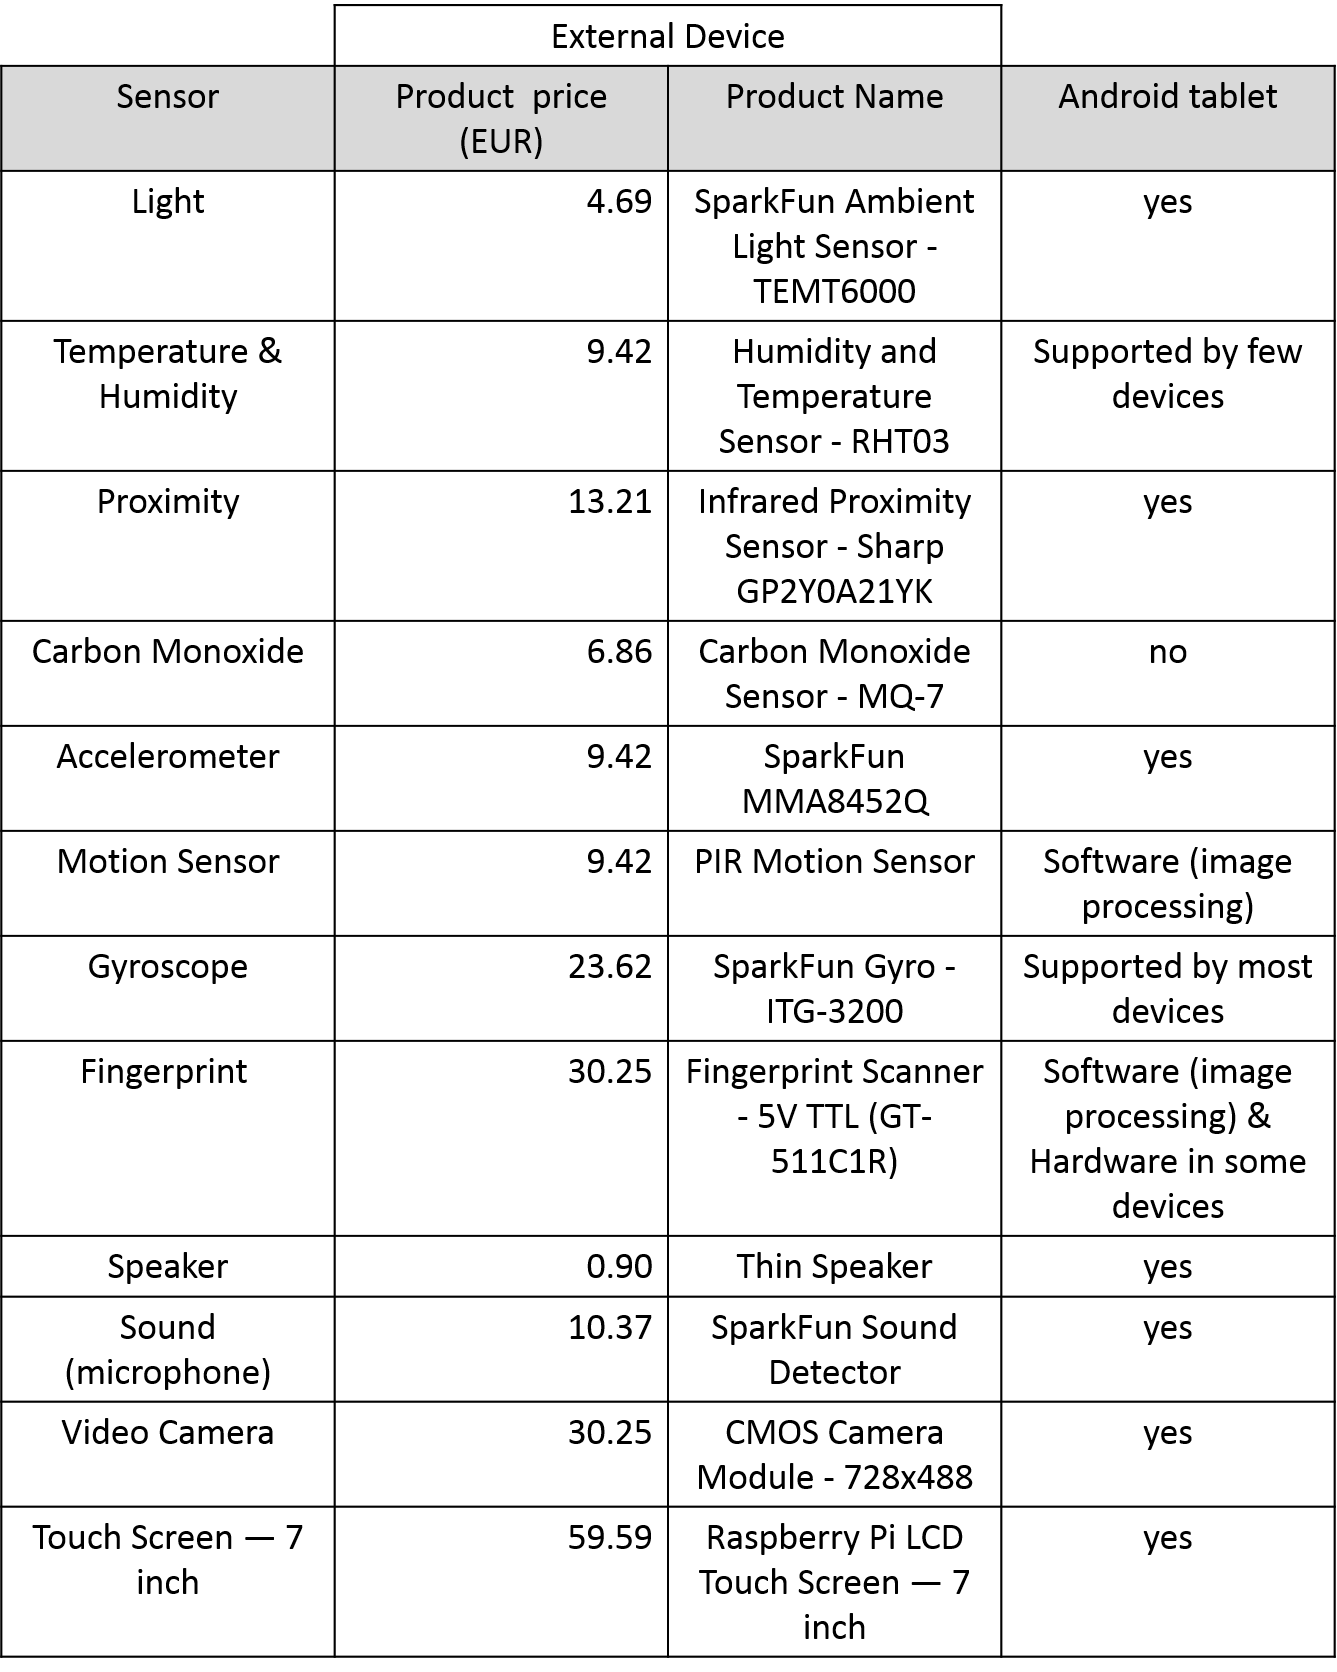
\includegraphics[width=0.7\textwidth]{Figures/table_sensors}
\caption{Android embedded sensors Vs Sensors for Arduino or Raspberry pi}
\label{table_sensors}
\end{figure}



